\documentclass[11pt]{article}
\usepackage[margin=1.4cm,a4paper,landscape]{geometry}
\usepackage{tikz}
\usepackage{xcolor}
\usepackage{lmodern}
\usepackage[T1]{fontenc}
\pagestyle{empty}

\definecolor{swred}{HTML}{D8382B}
\definecolor{pwr}{HTML}{D8382B}
\definecolor{gnd}{HTML}{222222}
\definecolor{spi}{HTML}{1F6FEB}
\definecolor{i2c}{HTML}{1F9D55}
\definecolor{espfill}{HTML}{FFE9CC}
\definecolor{dwfill}{HTML}{DCEAF7}
\definecolor{snsfill}{HTML}{E6F5EC}

\begin{document}
\begin{center}
{\LARGE\bfseries\color{swred} SafeWork --- Worker Node Wiring}\\[2pt]
{\small ESP32-S3 (4d\_systems\_esp32s3\_gen4\_r8n16) $\;\cdot\;$ DWM3000 (UWB) $\;\cdot\;$ MAX30102 $\;\cdot\;$ BNO08x $\;\cdot\;$ pins match \texttt{config.h}}
\end{center}

\vspace{2mm}
\noindent\hfill\resizebox{!}{12.2cm}{%
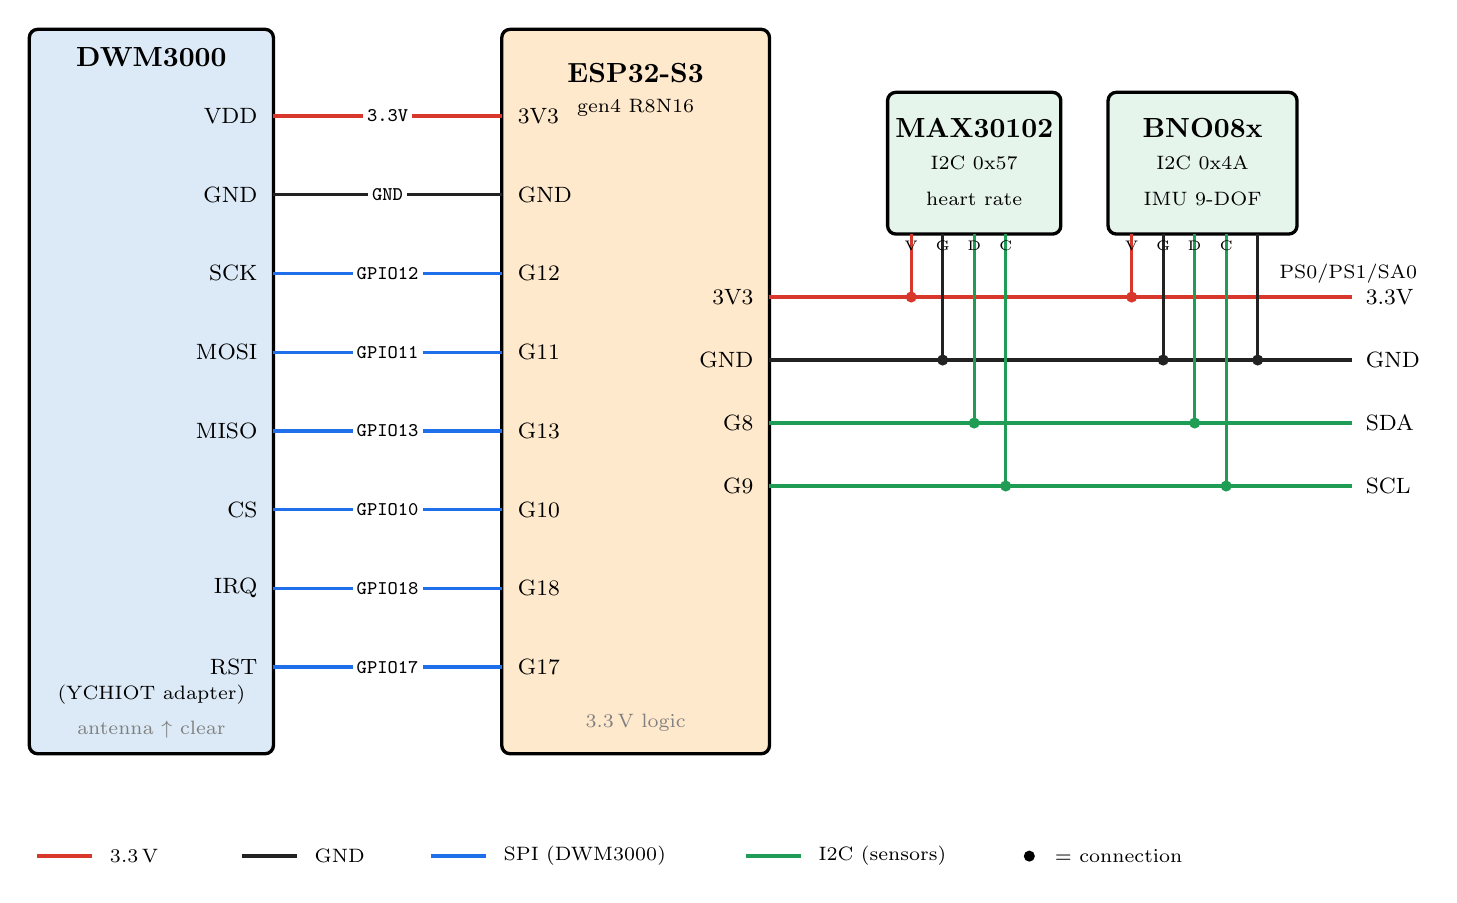
\begin{tikzpicture}[
  font=\small,
  chip/.style={draw, very thick, rounded corners=3pt},
  wpwr/.style={pwr, very thick},
  wgnd/.style={gnd, very thick},
  wspi/.style={spi, very thick},
  wi2c/.style={i2c, very thick},
  pin/.style={font=\footnotesize},
  glbl/.style={font=\scriptsize\ttfamily, fill=white, inner sep=1.5pt},
]

% ---------- ESP32-S3 (centre) ----------
\draw[chip, fill=espfill] (-1.7,-4.6) rectangle (1.7,4.6);
\node[font=\bfseries] at (0,4.05) {ESP32-S3};
\node[font=\scriptsize] at (0,3.6) {gen4 R8N16};
\node[font=\scriptsize, gray] at (0,-4.2) {3.3\,V logic};

% ---------- DWM3000 (left) ----------
\draw[chip, fill=dwfill] (-7.7,-4.6) rectangle (-4.6,4.6);
\node[font=\bfseries] at (-6.15,4.25) {DWM3000};
\node[font=\scriptsize] at (-6.15,-3.85) {(YCHIOT adapter)};
\node[font=\scriptsize, gray] at (-6.15,-4.3) {antenna $\uparrow$ clear};

% SPI + power rows: y, esp-pin, dw-pin, wire-style, gpio-label
\foreach \y/\ep/\dwp/\st/\gl in {
   3.5/3V3/VDD/wpwr/{3.3V},
   2.5/GND/GND/wgnd/{GND},
   1.5/G12/SCK/wspi/{GPIO12},
   0.5/G11/MOSI/wspi/{GPIO11},
  -0.5/G13/MISO/wspi/{GPIO13},
  -1.5/G10/CS/wspi/{GPIO10},
  -2.5/G18/IRQ/wspi/{GPIO18},
  -3.5/G17/RST/wspi/{GPIO17}}
{
  \draw[\st] (-1.7,\y) -- (-4.6,\y);
  \node[pin, anchor=west]  at (-1.62,\y) {\ep};
  \node[pin, anchor=east]  at (-4.68,\y) {\dwp};
  \node[glbl] at (-3.15,\y) {\gl};
}

% ---------- I2C rails (right) ----------
% rail y, esp-pin, style, right-label
\foreach \y/\ep/\st/\rl in {
   1.2/3V3/wpwr/{3.3V},
   0.4/GND/wgnd/{GND},
  -0.4/G8/wi2c/{SDA},
  -1.2/G9/wi2c/{SCL}}
{
  \draw[\st] (1.7,\y) -- (9.1,\y);
  \node[pin, anchor=east] at (1.62,\y) {\ep};
  \node[pin, anchor=west] at (9.15,\y) {\rl};
}

% ---------- MAX30102 ----------
\draw[chip, fill=snsfill] (3.2,2.0) rectangle (5.4,3.8);
\node[font=\bfseries] at (4.3,3.35) {MAX30102};
\node[font=\scriptsize] at (4.3,2.9) {I2C 0x57};
\node[font=\scriptsize] at (4.3,2.45) {heart rate};
% taps VIN,GND,SDA,SCL at x=3.5,3.9,4.3,4.7 down to rails 1.2,0.4,-0.4,-1.2
\draw[wpwr] (3.5,2.0) -- (3.5,1.2);   \fill[pwr] (3.5,1.2) circle (2pt);
\draw[wgnd] (3.9,2.0) -- (3.9,0.4);   \fill[gnd] (3.9,0.4) circle (2pt);
\draw[wi2c] (4.3,2.0) -- (4.3,-0.4);  \fill[i2c] (4.3,-0.4) circle (2pt);
\draw[wi2c] (4.7,2.0) -- (4.7,-1.2);  \fill[i2c] (4.7,-1.2) circle (2pt);
\node[font=\tiny] at (3.5,1.85) {V}; \node[font=\tiny] at (3.9,1.85) {G};
\node[font=\tiny] at (4.3,1.85) {D}; \node[font=\tiny] at (4.7,1.85) {C};

% ---------- BNO08x ----------
\draw[chip, fill=snsfill] (6.0,2.0) rectangle (8.4,3.8);
\node[font=\bfseries] at (7.2,3.35) {BNO08x};
\node[font=\scriptsize] at (7.2,2.9) {I2C 0x4A};
\node[font=\scriptsize] at (7.2,2.45) {IMU 9-DOF};
\draw[wpwr] (6.3,2.0) -- (6.3,1.2);   \fill[pwr] (6.3,1.2) circle (2pt);
\draw[wgnd] (6.7,2.0) -- (6.7,0.4);   \fill[gnd] (6.7,0.4) circle (2pt);
\draw[wi2c] (7.1,2.0) -- (7.1,-0.4);  \fill[i2c] (7.1,-0.4) circle (2pt);
\draw[wi2c] (7.5,2.0) -- (7.5,-1.2);  \fill[i2c] (7.5,-1.2) circle (2pt);
\node[font=\tiny] at (6.3,1.85) {V}; \node[font=\tiny] at (6.7,1.85) {G};
\node[font=\tiny] at (7.1,1.85) {D}; \node[font=\tiny] at (7.5,1.85) {C};
% PS0/PS1/SA0 -> GND
\draw[wgnd] (7.9,2.0) -- (7.9,0.4);   \fill[gnd] (7.9,0.4) circle (2pt);
\node[font=\scriptsize, anchor=west] at (8.05,1.5) {PS0/PS1/SA0};

% ---------- legend ----------
\begin{scope}[shift={(-7.6,-5.9)}]
  \draw[wpwr] (0,0)--(0.7,0);  \node[anchor=west,font=\scriptsize] at (0.8,0) {3.3\,V};
  \draw[wgnd] (2.6,0)--(3.3,0);\node[anchor=west,font=\scriptsize] at (3.4,0) {GND};
  \draw[wspi] (5.0,0)--(5.7,0);\node[anchor=west,font=\scriptsize] at (5.8,0) {SPI (DWM3000)};
  \draw[wi2c] (9.0,0)--(9.7,0);\node[anchor=west,font=\scriptsize] at (9.8,0) {I2C (sensors)};
  \fill (12.6,0) circle (2pt); \node[anchor=west,font=\scriptsize] at (12.8,0) {= connection};
\end{scope}

\end{tikzpicture}%
}

\vspace{3mm}
\begin{center}
\fbox{\parbox{0.95\textwidth}{\small
\textcolor{swred}{\textbf{POWER SAFETY}}: every VIN/VDD is \textbf{3.3\,V} (ESP32-S3 \texttt{3V3} pin), common GND ---
\textbf{never 5\,V / VIN / USB} (5\,V destroys the DWM3000). Measure the 3.3\,V rail with a meter and check
polarity \emph{before} inserting the module. \quad
\textbf{BNO08x}: tie PS0=PS1=GND for I2C mode, SA0=GND $\rightarrow$ 0x4A. \quad
\textbf{RSTn}: open-drain, never drive HIGH. \quad
\textbf{Anchor node} = ESP32-S3 + DWM3000 only (the SPI block above), no sensors.
}}
\end{center}

\end{document}
